\documentclass[11pt]{article}

\usepackage[margin=1in]{geometry}
\usepackage{amsmath,amssymb}
\usepackage{booktabs}
\usepackage{graphicx}
\usepackage{tikz}
\usetikzlibrary{arrows.meta,positioning}
\usepackage[hidelinks]{hyperref}

\title{Northline Outfitters: PDP Experiment}
\author{Jacqueling Ding}
\date{\today}

\begin{document}

\maketitle

\section*{Part A. Design}
\subsection*{A1. Estimand}

\paragraph{Treatment, unit, and outcome.}
The treatment is assignment to the redesigned product detail page (PDP),
with larger imagery, a sizing guide above the fold, and customer reviews
moved up from the footer. The control is assignment to the existing PDP.
The chosen unit is a customer, indexed by $i$ and identified by
\texttt{user\_id}; sessions are repeated observations within that unit.
The design assumes assignment persists across a customer's sessions, which
must be checked against the assignment information. The outcome is total
revenue in USD from that customer over the fixed two-week test window,
including zero for customers who make no purchases. It is neither revenue
per session nor revenue conditional on purchasing.

\paragraph{Potential outcomes and target population.}
Let $Z_i\in\{0,1\}$ denote assignment, and let $R_i(a)$ denote customer
$i$'s total two-week revenue under assignment to page $a$. Define
\[
Y_i(1)=R_i(\text{redesigned PDP}),
\qquad
Y_i(0)=R_i(\text{existing PDP}).
\]
Each potential outcome includes all sessions that would occur under its
respective assignment, so changes in visit frequency are part of the effect.
The target population $\mathcal{P}$ is customers eligible for the proposed
PDP rollout under the experiment's eligibility rules, including customers
who would not purchase. Eligibility should be defined before treatment,
rather than by subsequent purchasing or session counts. The estimand is
\[
\tau_{\mathcal{P}}
=\mathbb{E}_{i\sim\mathcal{P}}\!\left[Y_i(1)-Y_i(0)\right],
\qquad \text{measured in USD per customer over two weeks.}
\]

\paragraph{The VP's decision.}
The VP requires the average treatment effect (ATE) of offering the redesign
to the eligible rollout population, with a business threshold of
$\tau_{\mathcal{P}}\geq\$1.50$. Because treatment is defined as assignment,
this is an intention-to-treat (ITT) estimand: it includes any failures to
view or use the assigned page. Under full compliance, it also equals the
ATE of receiving the redesign. The ATT, an effect restricted to treated
customers, is not the policy target because rollout concerns all eligible
customers. Randomization identifies the assignment effect for the
experimental population; extending that effect to future rollout customers
requires that the experimental customers and conditions adequately represent
the rollout population and setting. A positive effect alone does not meet
the VP's requirement, and the eventual decision must account for uncertainty
relative to the \$1.50 threshold.

\paragraph{SUTVA.}
For each customer, two-week revenue depends only on that customer's own
assignment, not on other customers' assignments, and each arm represents a
well-defined page experience without hidden versions that change its effect.
Consistency then means the observed outcome is $Y_i=Y_i(Z_i)$. One possible
violation is shared inventory: if treated customers buy enough gear to cause
stockouts, control customers may lose purchasing opportunities. Their revenue
would then depend on other customers' treatment assignments.

\subsection*{A2. Assignment DAG}

Figure~\ref{fig:assignment-dag} represents the assignment and outcome process.
Here $X_i$ is a pre-treatment customer characteristic such as prior revenue,
$Z_i$ is randomized assignment to the redesigned PDP, $M_i$ is a
post-treatment response such as time on page or conversion, $U_i$ is latent
purchase propensity, and $Y_i$ is two-week customer revenue.

\begin{figure}[ht]
    \centering
    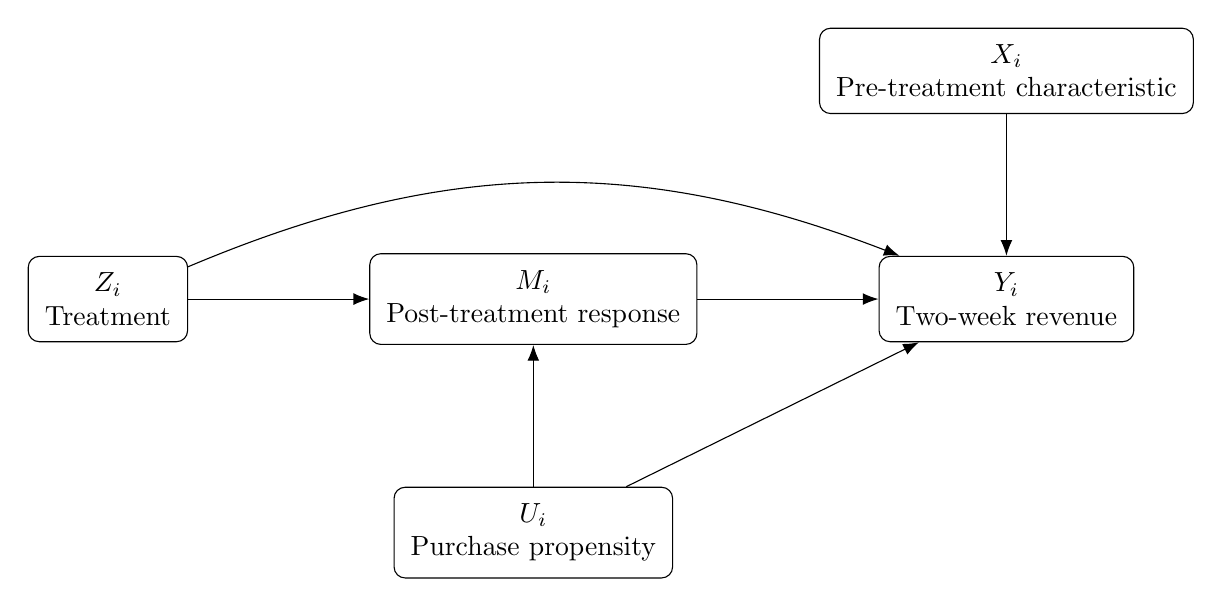
\begin{tikzpicture}[
        node distance=1.8cm and 2.3cm,
        every node/.style={draw, rounded corners, align=center, inner sep=6pt},
        >={Latex[length=2mm]}
    ]
        \node (z) {$Z_i$\\Treatment};
        \node (m) [right=of z] {$M_i$\\Post-treatment response};
        \node (y) [right=of m] {$Y_i$\\Two-week revenue};
        \node (x) [above=of y] {$X_i$\\Pre-treatment characteristic};
        \node (u) [below=of m] {$U_i$\\Purchase propensity};

        \draw[->] (z) -- (m);
        \draw[->] (z) to[bend left=22] (y);
        \draw[->] (m) -- (y);
        \draw[->] (x) -- (y);
        \draw[->] (u) -- (m);
        \draw[->] (u) -- (y);
    \end{tikzpicture}
    \caption{DAG for randomized PDP assignment.}
    \label{fig:assignment-dag}
\end{figure}

Random assignment leaves $Z_i$ with no incoming arrows, so it is independent
of both measured pre-treatment characteristics $X_i$ and unmeasured causes
$U_i$ of revenue. Therefore, under SUTVA, the difference in mean customer
revenue between assignment arms identifies the causal ATE without covariate
adjustment; pre-treatment covariates may still be used to improve precision.

The analysis must not condition on \texttt{converted}. It is a
post-treatment variable playing the role of $M_i$: conditioning on it would
block the mediated path $Z_i\rightarrow M_i\rightarrow Y_i$ and would also
open the collider path $Z_i\rightarrow M_i\leftarrow U_i\rightarrow Y_i$.
Either change destroys identification of the total effect represented by the
unadjusted randomized comparison.

\subsection*{A3. Randomization Unit}

The experiment randomized by \textbf{user}. The log contains 200,385 sessions
from 24,000 users; 22,166 users appear in multiple sessions, yet none appears
in both treatment arms, while every one of the four regions contains both
arms. Session randomization would expose repeat visitors to both pages, so a
session's outcome could depend on earlier assignments; that carryover would
violate the treatment definition and could bias a simple session-level
contrast for the all-redesign-versus-all-control customer effect. Moreover,
treating correlated sessions as independent would understate variance, and
cluster-robust inference would give up much of the apparent sample-size gain.
Region randomization would avoid within-customer contamination but would
leave only four independent clusters, producing poor covariate balance and
very high sampling variance; analyzing customers as independent would again
severely understate uncertainty and could turn region composition into an
apparent treatment effect. User assignment therefore matches the customer-
level estimand while retaining 24,000 independent randomization units.

\subsection*{A4. Power and Minimum Detectable Effect}

Following the project data definition, I treated \texttt{revenue\_14d} as the
pre-treatment 14-day revenue measure. I retained one observation per
randomized user and did not use session revenue or conversion. The resulting
baseline standard deviation is $s=\$161.55$, with
$n_T=n_C=12{,}000$. For a two-sided test with
$\alpha=0.05$ and power $1-\beta=0.80$, the normal-approximation MDE is
\[
\operatorname{MDE}
=(z_{1-\alpha/2}+z_{1-\beta})s
  \sqrt{\frac{1}{n_T}+\frac{1}{n_C}}
=(1.960+0.842)(161.55)\sqrt{\frac{1}{12{,}000}+\frac{1}{12{,}000}}
=\$5.84.
\]
With equal allocation, the total sample size required for an effect
$\delta=\$1.50$ is
\[
N
=\left\lceil
  \frac{(z_{1-\alpha/2}+z_{1-\beta})^2s^2}
       {\delta^2(0.5)(0.5)}
 \right\rceil
=364{,}149,
\]
or approximately 182,075 treatment and 182,074 control users. Thus, the
realized 24,000-user test was \textbf{not capable of answering the question it
was run to answer at conventional power}: its \$5.84 MDE substantially exceeds
the VP's \$1.50 threshold. Failure to reject a small or zero effect later
cannot establish that the redesign fails the business threshold, and this
power limitation must remain explicit in the final recommendation.

\section*{Part B. Analysis}
\subsection*{B1. Validity Checks}

All checks use one observation per randomized user. Following the project data
definition, \texttt{revenue\_14d} is treated as pre-treatment 14-day revenue.
The CSV contains \texttt{pre\_sessions\_56d} rather than
\texttt{pre\_sessions\_14d}, so I divided it by four to express the mean on a
14-day scale; this positive linear rescaling leaves its standardized difference
unchanged. Each balance statistic is the signed standardized difference,
treatment minus control. For continuous variables it is the difference in
means divided by the pooled standard deviation. For each categorical level it
is the difference in proportions divided by the pooled Bernoulli standard
deviation.

\paragraph{Sample ratio mismatch.}
The intended allocation was 50/50. The data contain exactly 12,000 treatment
and 12,000 control users. A Pearson chi-square goodness-of-fit test gives
$\chi^2(1)=0.00$ and $p=1.00$, so there is no evidence of a sample ratio
mismatch.

\begin{table}[ht]
    \centering
    \caption{Pre-treatment balance at the user level}
    \label{tab:balance}
    \begin{tabular}{lrrr}
        \toprule
        Characteristic & Treatment & Control & Std. difference \\
        \midrule
        Pre-revenue 14d (USD), mean & 94.49 & 90.69 & 0.024 \\
        Pre-sessions 14d, mean      & 8.35  & 8.28  & 0.011 \\
        Tenure (days), mean         & 517.48 & 518.25 & -0.002 \\
        Device: desktop             & 36.36\% & 37.76\% & -0.029 \\
        Device: mobile              & 63.64\% & 62.24\% & 0.029 \\
        Region: Midwest             & 19.63\% & 18.96\% & 0.017 \\
        Region: Northeast           & 21.68\% & 22.06\% & -0.009 \\
        Region: South               & 28.27\% & 28.48\% & -0.005 \\
        Region: West                & 30.43\% & 30.51\% & -0.002 \\
        \bottomrule
    \end{tabular}
\end{table}

Every absolute standardized difference is below 0.03, well inside the common
0.10 diagnostic threshold. The observed baseline characteristics therefore
show no meaningful imbalance between arms.

\paragraph{Missingness and duplicate identifiers.}
There are no missing values in any of the 12 columns. All 200,385
\texttt{session\_id} values are unique, and there are no duplicated
\texttt{user\_id}--\texttt{session\_id} pairs or exact duplicate rows.
Repeated \texttt{user\_id} values are expected because a customer can have
multiple sessions: 22,166 of the 24,000 users have more than one session.
No user appears in multiple arms, and the user-level fields used above are
constant across each user's sessions. Together, the SRM, balance, missingness,
and identifier checks reveal no data-validity warning for the randomized
comparison.

\subsection*{B2. Naive Estimate}

The naive analysis uses the file exactly as delivered: each of the 200,385
session rows is treated as an independent observation, and session revenue is
regressed on an indicator for the treatment arm,
\[
    \texttt{revenue}_{is}=\alpha+\tau_{\mathrm{naive}}Z_i+\varepsilon_{is}.
\]
There are 100,727 treatment sessions and 99,658 control sessions. Mean revenue
per session is \$11.2570 in treatment and \$10.9197 in control, producing
\[
    \widehat{\tau}_{\mathrm{naive}}=\$0.3373,
    \qquad
    \operatorname{SE}_{\mathrm{HC1}}(\widehat{\tau}_{\mathrm{naive}})=\$0.1398,
\]
with a 95\% confidence interval of $[\$0.0632,\ \$0.6114]$. This is a
session-weighted difference, and the HC1 standard error treats repeat sessions
from the same user as independent. It is therefore the requested hurried
benchmark, not yet an estimate or uncertainty measure aligned with the
customer-level estimand.

\subsection*{B3. Failure Mode and Corrected Estimate}

\paragraph{Diagnosis from the data.}
The B2 analysis commits pseudoreplication: treatment was randomized once per
user, but it treats every session as a new independent experiment. This is a
material feature of the data, not a hypothetical concern. Of the 24,000
users, 22,166 (92.4\%) have multiple sessions; the mean is 8.35 sessions, the
median is 7, and one user contributes 102 rows. Session count is also
associated with the outcome: its correlation with a user's total two-week
revenue is 0.507. Thus, the rows within a user share customer-specific revenue
propensity, and a session-level mean gives frequent visitors more weight than
customers with few visits.

HC1 permits unequal error variances across rows, but it still treats the rows
as independent. Positive within-user dependence therefore makes 200,385 rows
look more informative than the 24,000 independent randomized units. This
biases the inference toward excess precision: standard errors are too small,
confidence intervals are too narrow, and statistical significance is too
easy to obtain. The data demonstrate the direction directly. Holding the B2
session-level coefficient fixed at \$0.3373 and changing only its covariance
estimator gives:

\begin{table}[ht]
    \centering
    \caption{Uncertainty for the same session-level coefficient}
    \label{tab:se-comparison}
    \begin{tabular}{lr}
        \toprule
        Standard-error estimator & Standard error \\
        \midrule
        Naive HC1, sessions treated as independent & \$0.1398 \\
        Cluster-robust by randomized user           & \$0.2154 \\
        \bottomrule
    \end{tabular}
\end{table}

The user-clustered standard error is 1.54 times the naive one, or 54.0\%
larger. Equivalently, the naive standard error is 35.1\% below the corrected
standard error. This comparison is made on the identical coefficient so that
the units are the same. Clustering fixes the B2 covariance, but it does not
change B2's session-weighted estimand.

\paragraph{Corrected customer-level analysis.}
To estimate the target effect, I summed session revenue within each user and
then compared the 12,000 treatment-user totals with the 12,000 control-user
totals. This gives every randomized user equal weight. Mean two-week revenue
is \$94.49 for treatment users and \$90.69 for control users, so
\[
    \widehat{\tau}_{\mathrm{user}}=\$3.804,
    \qquad
    \operatorname{SE}_{\mathrm{HC1}}(\widehat{\tau}_{\mathrm{user}})=\$2.085,
\]
with a 95\% confidence interval of $[-\$0.283,\ \$7.892]$. The point estimate
exceeds the VP's \$1.50 threshold, but the interval contains both zero and
\$1.50. The experiment therefore does not determine with conventional
precision whether the redesign clears the business threshold, consistent
with the power limitation identified in A4.

\subsection*{B4. CUPED Variance Reduction}

The corrected specification remains at the randomized-user level, with
$Y_i$ equal to total revenue summed over customer $i$'s sessions. Before
adjusting, I checked which revenue variable is genuinely pre-treatment. For
every one of the 24,000 users, \texttt{revenue\_14d} equals the sum of session
\texttt{revenue} exactly: the maximum absolute difference is zero and the
correlation is one. It is therefore the two-week outcome recorded redundantly
on each session row, not a valid CUPED covariate. Adjusting for it would amount
to controlling for the outcome itself and would produce meaningless perfect
``variance reduction.'' I instead use \texttt{pre\_revenue\_56d}, the field
explicitly measured before treatment. Dividing it by four would only rescale
its regression coefficient and would not change the adjustment.

The CUPED-equivalent ANCOVA is
\[
Y_i=\alpha+\tau_{\mathrm{CUPED}}Z_i
    +\theta\left(X_i-\bar X\right)+\varepsilon_i,
\]
where $X_i=\texttt{pre\_revenue\_56d}_i$. The pre-period outcome is strongly
predictive of the test-period outcome, with correlation 0.688. The treatment
group happened to have slightly lower mean pre-period revenue than control
(\$360.44 versus \$367.29), so adjustment raises the estimated effect from
\$3.804 to
\[
\widehat{\tau}_{\mathrm{CUPED}}=\$5.068,
\qquad
\operatorname{SE}_{\mathrm{HC1}}=\$1.510,
\]
with a 95\% confidence interval of $[\$2.108,\ \$8.027]$.

Relative to the corrected unadjusted standard error of \$2.085, the estimated
variance reduction is
\[
1-\frac{1.510^2}{2.085^2}=47.6\%.
\]
If this adjustment had been specified before the experiment, the corresponding
MDE would have been
\[
\operatorname{MDE}_{\mathrm{CUPED}}
=\operatorname{MDE}_{A4}
 \sqrt{\frac{\operatorname{Var}(\widehat\tau_{\mathrm{CUPED}})}
              {\operatorname{Var}(\widehat\tau_{\mathrm{unadjusted}})}}
=\$5.84\sqrt{1-0.4758}=\$4.23.
\]
CUPED lowers the A4 MDE by 27.6\%, from \$5.84 to \$4.23, but \$4.23 still
substantially exceeds the VP's \$1.50 threshold. Planning CUPED from the start
would have made this experiment more informative, but it would not have made
the design adequately powered to detect a threshold-sized effect.

\subsection*{B5. Randomization Inference}

For the sharp null $H_0:Y_i(1)=Y_i(0)$ for every user, I held the 24,000
observed user-level revenue totals fixed and performed 10,000 random
reassignments of exactly 12,000 users to treatment. Using the absolute
difference in mean user revenue as the test statistic and the standard
plus-one Monte Carlo correction, 688 permutations were at least as extreme as
the observed \$3.804 effect, giving a two-sided randomization-inference
$p$-value of 0.0689 (Monte Carlo standard error 0.0025).

The analytical HC1 $p$-value from B3 is 0.0681, only 0.0008 lower. The two
approaches therefore agree to within simulation error, and neither rejects
the sharp null at the 5\% level.

\section*{Part C. The Recommendation}
\subsection*{C1. Recommendation to the VP of Product}

\noindent
\textbf{Keep testing; do not ship the redesigned page yet.} The decision rests
on the average additional revenue generated per eligible customer during the
two weeks after assignment. Our best adjusted estimate is a \$5.07 increase
per customer, but this test was too small to reliably distinguish effects near
your \$1.50 break-even requirement: even with the revenue adjustment, it was
built to detect increases of roughly \$4.23 or more. The single assumption
that most threatens this conclusion is that one customer's assigned page did
not affect another customer's opportunity to buy; inventory stockouts caused
by the redesign, for example, would contaminate the comparison. One result
would change my recommendation: a larger follow-up test, using the same
customer-level assignment and a revenue adjustment specified before launch,
whose conservative lower estimate is above \$1.50 per customer. Until that
result is available, maintaining an expensive second template is not supported
by evidence precise enough for the stated business rule.

\subsection*{C2. Full-Rollout Threat}

The main threat at 100\% traffic is that the redesign's larger images and added
content could strain delivery systems and slow the page, reducing purchases in
a way the 50\% test did not reveal. I would monitor page-load time, error rate,
and abandonment and purchase rates by device during a staged ramp to detect
whether performance worsens as traffic increases.

\end{document}
